Java is an open source high-level, general-purpose(hard \& used to develop any kind of programs), object oriented language. If you wanna be a software developer than you must learn that 4 languages:-
\begin{enumerate}
	\item Python
	\item Java
	\item JavaScript
	\item C / C++
\end{enumerate}
In those, Java is second dominant (and popular also) language that you must learn if you wanna be a platform-independent developer. Also:-
\begin{itemize}
	\item[$\rightarrow$] Java has huge online community for getting help.
	\item[$\rightarrow$] Can be used in android development that is most preferable thing today.
\end{itemize}

\paragraph{Gosling explains his motivation for creating \textbf{JAVA}:}
James Gosling, father of \textbf{JAVA}. It is one of the world's most widely used programming language. It used over ten billion of devices and become central to the development of Android at Google. According to \textbf{Oracle}, there are $51$ billion active Java Virtual Machines deployed globally.

Java has two types of error. Syntax error and Semantic error. Syntax error is grammatical error and semantic error is that the line has no meaning.
\begin{itemize}
	\item[$\rightarrow$] "I are playing" - that's the syntax error.
	\item[$\rightarrow$] "He is hello" - this line has no meaning, semantic error.
\end{itemize} %%% Till here on original Java LaTeX document. %%%
\begin{center}
	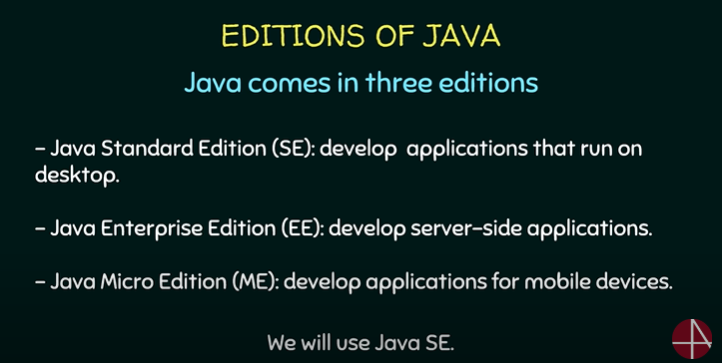
\includegraphics[width=200pt]{Source Images/Editions of Java.png} 
\end{center}

\section{IntelliJ IDEA: The IDE} % All OK.
\begin{wrapfigure}{r}{0.25\textwidth}
	
\includegraphics[width = 0.9\linewidth]{Source Images/IntelliJ IDEA user interface.png} 
\end{wrapfigure}

\textbf{IntelliJ IDEA} is the greatest \textbf{IDE} for writing and compiling Java source codes. Here in table \ref{IntelliJ IDEA:1} has some command and shortcuts of \textbf{IntelliJ IDEA} that are applicable to windows operating system.

\begin{center}
\rowcolors{3}{green!35}{green!70}
\arrayrulecolor{white}
	\begin{longtable}{|| m{1 em} || m{15 em} m{17 em} ||}
	\label{IntelliJ IDEA:1}\\
		\hline\hline
		\rowcolor{teal!20}
		\multicolumn{3}{c}{\textbf{\textsf{\textcolor{black}{IntelliJ IDEA Commands and Shortcuts}}}}\\
		\hline\hline
		1 & Debug Program & shift + f9\\
		\hline
		2 & Run Program & shift + f10\\
		\hline
		3 & Format Codes & ctrl + alt + L\\
		\hline
		4 & public static void main() & main / psvm\\
		\hline
		5 & System.out.println() & sout\\
		\hline
		6 & To warp a code block in a construct & ctrl + alt + T\\
		\hline
		7 & Search anything in project & double click shift (For a technical reason, I turned off the system)\\
		\hline
		8 & Invoke commit changes dialog & ctrl + K\\
		\hline
		9 & Select several words and edit together & press and hold shift + alt and double click on the word.\\
		\hline
		10 & Fill the code construct & start typing method declaration and press ctrl + shift + enter\\
		\hline
		11 & Join two statement in one line and remove unnecessary spaces & ctrl + shift + J\\
		\hline
		12 & Jump highlighted syntax error & f2 / shift + f2\\
		\hline
		13 & ctrl + shift + E & recently viewed or changed code fragment\\
		\hline
		14 & Change name of the function from main method & highlight method name then press shift + f6 and re-write\\
		\hline
		\rowcolor{red}
		15 & Quick scheme & view | Quick Switch Scheme or ctrl +  \\
		\hline
		16 & To evaluate any expression while debugging program & select the expression in the editor and press Alt + F8\\
		\hline
		17 & Create a new class & alt + ins (Now, not working perfectly)\\
		\hline
		18 & To see all the live template that are valid for this current method or context & ctrl + J (Close this by pressing "esc")\\
		\hline
		19 & Complete syntax with dot from code completion helper(highlighted) & ctrl + dot\\
		\hline
		20 & To close all editor tabs except current one & keep alt pressed and click cross button of current tab\\
		\hline
		21 & To see how to call an action & ctrl + shift + A\\
		\hline
		22 & To select multiple fragment in column mode & press alt + shift + insert and then hold ctrl + shift + alt and drag the mouse\\
		\hline
		23 & Rename an identifier and change all uses of it & Look at the leftmost side(gutter), here is a pencil marker. Click on this and click again Rename.\\
		\hline
		24 & To select a block of code & Double click of its opening brace.\\
		\hline
		25 & Invoke rename action box & mark down the field and press shift + f6\\
		\hline
		26 & Move statement up/down in current block only & put cursor at the end of the statement and hold shift + ctrl then press uparrow/downarrow\\
		\hline
		27 & Move line up/down at any place & shift + alt + up/down\\
		\hline
		28 & To scroll a file horizontally & Turn the mouse wheel while keeping Shift pressed\\
		\hline
		29 & Compare to different directories & select the file on form project (Press and hold shift and then one click on the directory) and press ctrl + D\\
		\hline
		30 & To delete the whole line at the caret & ctrl + Y\\
		\hline\hline
	\caption{Commands and Shortcuts: Intellij IDEA}
	\end{longtable}
\end{center}

\pagebreak

\section{Syntax Difference between \textcolor{blue!90}{C++} and \textcolor{blue!90}{Java}}
\begin{table}[h!] % h! : In-place command.
	\arrayrulecolor{black}
	\centering
	\begin{tabular}{|| c | c ||}
		\hline
		\textbf{\textcolor{blue}{C++}} & \textbf{\textcolor{blue}{Java}}\\
		\hline\hline
		string & String\\
		\hline
		int main() & public static void main()\\
		\hline
		empty() & isEmpty()\\
		\hline
		vector & ArrayList()\\
		\hline
	\end{tabular}
	\caption{Syntax Difference between \textcolor{blue!90}{\huge C++} and \textcolor{blue!90}{\huge Java}}
\end{table}

\section{Object Oriented Programming (OOP) with \textbf{JAVA}}
As I mentioned, Java is full object oriented language and do not provide low level programming features like pointer, operator overloading etc. as C / C++ does. Every byte of code of Java are written in a class with same name of that file. Now, what is object? An object is a collection of data (of primitive type) belongs to a class and that class provides methods for manipulate this object. So, Java is "object-oriented" means it uses object to represent data and provide methods related to them. To create a new object in Java, must use new keyword. Java has a huge amount of built-in classes, \textbf{Point} and \textbf{Rectangle} are two of them. You can see details of that two classes from oracles Java documentation. As we know from previous section, some of same type classes are wrapped in a package. Point class is belongs to \textbf{awt} package of Java source code library. Variables that belong to an object are usually called \textbf{attribute}, but you might also see them called \textbf{fields}. Both are correct. To access an attribute of an object, Java uses \textbf{dot notation}. Syntax:- \\
\begin{lstlisting}[language = java]
	dataType variable = objectName.attribute;
\end{lstlisting}
Objects are pass by reference to the method. In Java, keyword \textcolor{blue}{null} means "No Objects". When you try to use a null value, \textbf{NullPointerException} will be thrown. But you can return or send a null value to a method.

\section{Arrays Class}
Arrays class are used to manipulate arrays. Arrays class is a member of the java Collections Framework. We can initialize Array like this, \texttt{int anArray[];} which is not conventional way.\\
Iterate over array by a stream:\\
\texttt{\footnotesize Arrays.stream(new int[] {1, 2, 3}).forEach(n -> System.out.print(n + " "));}
\subsection{parallelSort() Method}
Java 8 introduced a new method called \textbf{parallelSort()} in java.util.Arrays class. If uses parallel sort algorithm. This method uses "MultiThreading" which makes the sorting faster as compared to normal sorting method. This is a void method. Time complexity $O(n\log(n))$
\paragraph{Algorithm for parallelSort():}
	\begin{enumerate}
		\item The array is divided into sub-arrays and that sub-array is again divided into their sub-arrays. Until the minimum level of detail in a set of array.
		\item Arrays are sorted individually my multiple thread.
		\item This algorithm uses Frok / Join concept for sorting.
		\item Sorted sub-arrays are then merged.
	\end{enumerate}

\section{Matcher Class}
Reference: \href{https://docs.oracle.com/javase/7/docs/api/java/util/regex/Matcher.html}{Oracle Help Center}\linebreak
I have written some descriptions for this class in my Java notebook.

\paragraph{Package}
java.util.regex
\paragraph{Properties}
An engine that perform match operations on a character sequence by interpreting patter(Such a regular expression or regex.)

\section{Interface}
Interface is a feature that implements most futuristic class. In java programming language, an interface is a reference type, similar to a class, that can contain only constants, method signatures, default methods, interfaces cannot be instantiated - they can only be implemented by classes or extended by other interfaces. Extension is discussed later in this lesson. All method had just signature but not method body. Methods signature are terminated with a semicolon.

\section{Anonymous Class}
Anonymous class enables you to make your code more concise. They enable you to declare and instantiate a class at the same time. They are look like local classes except that they don't have a name.\hfill
Use them if you need to use a local class only once.

\section{Lambda Expression}
Lambda Expression enables you to pass functionality as an argument to another method. Such as, what action should be taken when someone clicks a button.
\paragraph{Note of Collection:}A \textcolor{blue}{Collection} is an object that groups multiple elements into a single unit by a wrapper class for primitives and instant class for local class objects. Collections are used to store, retrieve, manipulate and communicate aggregate data. As, a \textcolor{blue}{List} is an \textcolor{blue}{Collection} of ordered type.

\section{Object Ordering}
\begin{framed}
	\begin{lstlisting}[language = java]
		Collections.sort(list)
	\end{lstlisting}
\end{framed}
\paragraph{Starting:}
\begin{multicols}{2}
There is an interface named \textit{\textcolor{blue}{Comparable}} and has a \textit{\textcolor{blue}{compare}} method at this. we can use(override) this method for our own manipulation of sorting / ordering. \textsf{Comparable} implementations provide a \textit{natural ordering} for a class, which allows objects of that class to be sorted automatically.\linebreak
If you try to sort a list, which don not implement Comparable, will throw a \textbf{\textcolor{blue}{ClassCastException}}. Similarly, \textit{Collections.sort(list)} will throw the same exception if we try to sort that list whose elements cannot be compared to one another.
\end{multicols}
\begin{quotation}
	Elements that can be compared to one another are called \textit{mutually comparable}.
	\begin{flushright}
		- Oracle
	\end{flushright}
\end{quotation}

\subsection{Implement own comparable type}
The comparable interface consist of the following methods:
\begin{lstlisting}
	public interface Comparable<T>
	{
		public int compareTo(T o);
	}
\end{lstlisting}

This method compares the receiving object with the specified object and returns negative, zero or positive value depending on whether the receiving object is less than, equal or greater than the specified object.
\begin{lstlisting}[language = java, backgroundcolor = \color{white}]
public class Name implements Comparable<Name>
{
    private final String firstName, lastName;

    public Name(String firstName, String lastName)
    {
        if (firstName == null || lastName == null)
            throw new NullPointerException();

        this.firstName = firstName;
        this.lastName = lastName;
    }

    public String firstName() {return firstName;}
    public String lastName() {return lastName;}

    public boolean equals(Object o)
    {
        if (!(o instanceof Name))
            return false;

        Name n = (Name) o;
        return n.firstName.equals(firstName) && n.lastName.equals(lastName);
    }

    public int hashCode()
    {
    	return 31 * firstName.hashCode() + lastName.hashCode();
    }
    public String toString() {return firstName + " " + lastName;}

    public int compareTo(Name n)
    {
        int lastCmp = lastName.compareTo(n.lastName);
        return (lastCmp != 0 ? lastCmp : firstName.compareTo(n.firstName));
    }
}
\end{lstlisting}

\subsection{Comparators}
What if you want to sort some objects in an order other than their natural ordering? Or what if you want to sort some objects that don't implement Comparable? To do either of these things, you'll need to provide a Comparator - an object that encapsulates an ordering. The Comparator interface consists of a single method:
	\begin{lstlisting}
		public interface Comparator<T>
		{
			int compare(T o1, T o2);
		}
	\end{lstlisting}

The \textit{compare} method returns less than zero, zero or greater than zero depending on whether the first argument is less than, equal or greater than the second.
\paragraph{By GeeksforGeeks:}
A \textit{comparator} is an interface\footnote{That just had a face, no body.} that used to order the objects of user-	defined classes. A \textit{comparator} object is capable of comparing two objects of two different classes. Suppose we have an "ArrayList" of objects containing fields like \textsc{Name, Roll, Section} and we need to sort the "ArrayList" based on \textsc{Roll}. We can do this by:
	\begin{enumerate}
		\item[Method 1:] One obvious approach is to write our own "sort()" function using one of the standard algorithm. This approach require rewrite the entire function.
		\item[Method 2:] Using \textit{comparator} interface\footnote{Present in java.util package.}. It contains two method signature:-
		\begin{enumerate}
			\item compare(Object o1, Object o2);
			\item equals(Object element);
		\end{enumerate}
	\end{enumerate}
	
\subparagraph{How does "Collections.sort()" work?}
Internally the "sort()" method calls Compare method of that class and asks for "which is grater?". Then compare method returns $-1, 0$ or $1$ based on compared object. It uses this result to then determine if they should be swapped for its sort.
\subparagraph{A working program:}
A working program from geeksforgeeks
\begin{lstlisting}[language = java, caption = Comparator for sorting Student class, backgroundcolor = \color{white}]
class Student
{
    String name, address;
    int roll;

    public Student(String name, int roll, String address)
    {
        this.name = name;
        this.roll = roll;
        this.address = address;
    }

    public String toString()
    {
        return this.name + " " + this.roll + " " + this.address;
    }
}

class SortByName implements Comparator<Student>
{
    public int compare(Student s1, Student s2)
    {
        return s1.name.compareTo(s2.name);
    }
}

class SortByAddress implements Comparator<Student>
{
    public int compare(Student s1, Student s2)
    {
        return s1.address.compareTo(s2.address);
    }
}

class Main
{
    public static void main(String[] args)
    {
        ArrayList<Student> list = new ArrayList<>();
        list.add(new Student("Kiron", 65, "Madaripur"));
        list.add(new Student("Miron", 73, "Faridpur"));
        list.add(new Student("Chiron", 11, "Dhaka"));

        Collections.sort(list, new SortByName());
        for (int i = 0; i < list.size(); i++)
            System.out.println(list.get(i));

        System.out.println();
        Collections.sort(list, new SortByAddress());
        for (int i = 0; i < list.size(); i++)
            System.out.println(list.get(i));
    }
}
\end{lstlisting}

\begin{tcolorbox}[enhanced, title = Output, attach boxed title to top left, width = 5 cm]
	Chiron 11 Dhaka\\
	Kiron 65 Madaripur\\
	Miron 73 Foridpur\\
\vspace{2.5 mm}
	Chiron 11 Dhaka\\
	Miron 73 Foridpur\\
	Kiron 65 Madaripur\\
\end{tcolorbox}

Just change the return value inside compare method, that will allow us to sort objects in required manner. e.g. for descending order, swap the position of objects.

\paragraph{Again Oracle:}
\section{Math Class}
\subsection{Beyond Math Class}
The "Math" class in \textit{java.lang} package provides methods and constants for doing more advance mathematical computation. All the methods in "Math" class are "static", so they can be called directly. Using the \textbf{\textcolor{blue}{static import}} language feature, you don't have to write Math in front of every math function.
\begin{lstlisting} [language = java]
	import static java.lang.Math.*;
\end{lstlisting}

* will import all the methods from the "Math" class.\\
Now we can write code like this:
\subsection{Constants and Basic Methods}
The class contains two constants:
	\begin{enumerate}
		\item[Math.E] Base of natural logarithms.
		\item[Math.PI] Ratio of the circumference of a circle to its diameter.
	\end{enumerate}
	
This class also includes more than 40 static methods.
	
\subsection{Random Numbers}
The random() method returns a pseudo-randomly selected number between 0.0 and 1.0
	\begin{enumerate}
		\item primitive abs(primitive arg) Returns the absolute value of "arg".
		\item ceil()
		\item floor()
		\item double rint(double d) Returns the integer that is closest in value to the argument as double.
		\item min(a, b);
		\item max(a, b);
		\item double exp(double d);
		\item double log(double d);
		\item pow(base, exponent);
		\item sqrt(double d);
		\item All trigonometric methods.
		\item double atan2(double y, double x) Converts rectangular coordinates (x, y) to polar coordinate (r, $\theta$) and returns $\theta$.
		\item double toDegrees(double d);
		\item double toRadians(double d);
		\item con(angle)
	\end{enumerate}

\section{Graph}

\subsection{Representation}

\paragraph{What is graph:}
Graph is a collection of nodes / vertices(\textbf{V}) and edges(\textbf{E}) placed between them. Represented as: $$G = (V, E)$$ We can traverse vertices through edges. These edges might be weighted or non-weighted.

\subparagraph{There are two kinds of graphs:}
	\begin{itemize}
		\item[Un-directed:] Not direction specified. We can traverse either direction between two vertices.
		\item[Directed:] Can traverse only in the specified direction between that two vertices.
	\end{itemize}
\tikzset
{
	VertexForGraph/.style = {draw, circle, very thick, black, fill = teal!30}
}
\begin{center}
	\tikz
	{
		\node(0) at (-1, 2) [VertexForGraph] {A};
		\node(1) at (2 ,2) [VertexForGraph] {B};
		\node(2) at (4.5, 0.5) [VertexForGraph] {C};
		\node(3) at (2, -1) [VertexForGraph] {D};
		\node(4) at (-1, -1) [VertexForGraph] {E};
	
		\draw (0) -- (1);
		\draw (1) -- (2);
		\draw (1) -- (3);
		\draw (1) -- (4);
		\draw (2) -- (3);
		\draw (3) -- (4);
		\draw (4) -- (0);
	}
\end{center}
	
Two common ways to represent a graph:
	\begin{itemize}
		\item Adjacency Matrix
		\item Adjacency List
	\end{itemize}

\paragraph{Adjacency Matrix:}
Adjacency matrix is a 2D array which had the size of\\$(V$ $*$ $V)$, where $V$ are the number of vertices in the graph. Adjacency matrix is symmetric if the graph is un-directed. Here is the adjacency matrix for above graph:
	\begin{table}[h!]
		\centering
		\begin{tabular}{c c c c c c}
			  & A & B & C & D & E\\
			A & 0 & 1 & 0 & 0 & 1\\
			B & 1 & 0 & 1 & 1 & 1\\
			C & 0 & 1 & 0 & 1 & 0\\
			D & 0 & 1 & 1 & 0 & 1\\
			E & 1 & 1 & 0 & 1 & 0\\
		\end{tabular}
	\end{table}

\section{Find Integer Root}
I got a problem from \textit{Leetcode} online judge. That wanna from us an integer root. Here is some attempt to reach the solution.

\paragraph{Natural Number}
In mathematics, the natural numbers are those used for counting\footnote{There are \textit{six} coins on the table: Cardinal Numbers} and ordering\footnote{This is the \textit{third} largest city in the world: Ordinal Numbers}. Normally natural numbers starts from $0$ and run as:- $1, 2, 3, 4,\dots$

\paragraph{Integer square root}
In number theory, the \textit{integer square root} $isqrt(n)$ is a positive integer $m$ where $m <= n$. Or, $$isqrt(n) = \lfloor\sqrt{n}\rfloor$$